\chapter{Introduction}
\label{chap:introFOR}
\minitoc\mtcskip

\lettrine[lines=3]{A}{s the years pass by,} information and communication technology (ICT) systems 
are becoming more and more pervasive in our lives, having 
a crucial role to play in countless industry, communication, security, cybernetics areas and applications.
%
Embedded systems are employed for critical purposes, 
such as air traffic and railway control, telephone networks and nuclear plants monitoring.
Security protocols are at the basis of e-commerce websites and services,
and are exploited in all applications committed to ensure user privacy.
Biomedical instruments and equipment are endowed with
automatic or proactive functionalities, %clearly fault-intolerant, 
%which have to automatically perform a task, 
and are supposed to help humans and prevent human error.

The essential requirements of safety, reliability and correctness for these systems suggest
(or, rather, compel)
to support their development, throughout the phases of the life cycle, %steps, namely, design, implementation, verification, and testing, 
by structured methodologies founded on \emph{formal methods}, %---some of them are even becoming integral part of standards---as  well as by suitable specification languages and automatic verification techniques and tools,
with the aim to provide effective verification techniques and tools, and reduce the verification time, while simultaneously increasing coverage.

The typical techniques of system engineering for system validation, namely, \emph{simulation} and \emph{testing}, 
are clearly not sufficient alone nowadays. They are dynamic techniques: 
the former involves performing some experiments with a restrictive set of scenarios or over a model, 
the latter actually running the system, whose correctness is determined by forcing it to traverse a set of execution paths. However, an exhaustive consideration of all execution paths is practically unfeasible, and thus testing and simulation can never be complete, that is, they can only show the presence of errors, but \emph{not their absence}.
Moreover, their effectiveness decreases dramatically as the complexity of design grows, 
they often discover errors and unpredictable behaviors in systems at late stages of development (or even when they have already been deployed), and are not effective at determining the more subtle and hidden bugs.
Just to mention a few of them, some famed examples of bugs which were discovered too late---so to speak---were those affecting, with catastrophic economic, functional, security or life consequences, the Intel Pentium CPU floating-point division unit~\cite{pratt1995}, the Ariane 5 rocket~\cite{jazequel1997}, the radiation therapy machine Therac 25~\cite{thomas1994}, the Needham-Schroeder authentication protocol~\cite{Lowe1996} and the ISDN protocol~\cite{holzmann1994}.

\emph{Formal methods}
are complementary to simulation and testing.
They can be considered as ``the applied mathematics for modeling and analyzing ICT systems''~\cite{Baier2008}, being their aim to establish system correctness with mathematical rigor. As a matter of fact,
\emph{all the possible states and scenarios of a system} are considered during formal verification, in order to prove that the system features some desired properties such as deadlock freedom, data integrity, liveness, safety, fairness, responsiveness, interference freedom, and so on.
The two most famous approaches to formal verification are \emph{axiomatic reasoning}  and \emph{model checking}.

Axiomatic reasoning involves specifying the desired properties of a system by means of \emph{formulas} of some logic; then a \emph{proof system}, consisting of axioms and rules, allows one to formally prove that the system meets the expected behavior. A well-known example is Hoare's tuple-based proof system. 
%
However, axiomatic reasoning has several limitations:
the proof rules are designed only for an \emph{a posteriori} verification of existing software, not for its systematic development; 
it is very time-consuming, cumbersome, and can be performed only by experts. As a consequence, it is mostly employed for (parts of) critical systems or security protocols.%
\footnote{Or to verify model checkers!}
Additionally, such techniques were developed having in mind  \emph{transformational} systems/programs:
in the 70s most early computer programs were designed to \emph{compute} something (i.e., transforming initial data to final ones), and correctness was to be assessed by showing that, given some preconditions on the input, desired post-conditions hold on the output of the program. The first tools of \emph{computer-aided verification}, namely, theorem provers, made their debut then, with the objective of automating mathematical logical reasoning. The language of such tools was often indeed Hoare-like. However, proofs could not be completely automated, and thus theorem provers were rather proof assistants and checkers.

In the 80s the focus shifted to \emph{reactive systems}, whose goal is
continuously interacting with the environment within
which they operate, instead of terminating their execution returning some value
(e.g., operating systems, communication protocols, programs
for process control, embedded systems). 
%The behavior of these systems is instead described 
% in terms of state-transition graphs, 
% whose nodes represent
% system states
% and are labeled with information true at
% that state. The edges represent
% system transitions
% as the result of some action of the system.
% Therefore paths (traces) represent system evolution (possible computations) as a sequence of states and transitions between states.
One of the most successful techniques for the verification of such systems is \emph{model checking}, on which research actively started during the early 80s, and originated from the independent work of Clarke and Emerson~\cite{CE81} and Queille and Sifakis~\cite{Queille1982}.

\section{An overview on MC}
In model checking (MC)~\cite{CE81,CGP02,VW86b,Queille1982} some properties of a %finite-state transition 
system are expressed in a \emph{temporal logic} (e.g., $\CTL$ or $\LTL$) and then verified over a model of the system itself (usually a labeled state-transition graph or Kripke structure) through \emph{exhaustive}---implicit or explicit---enumeration of all the reachable states. This technique is \emph{fully automatic}: MC algorithms
either terminate positively (proving that all properties are met), or produce a \emph{counterexample} (namely, a behavior that falsifies a property), which is extremely useful for debugging purposes.

Typical system properties that are to be checked over system models by MC algorithms are:
\begin{itemize}
	\item \emph{functional correctness} (``the system does what it is supposed to do'');
	\item \emph{safety} (``something bad never happens'');
	\item \emph{liveness} (``something good will eventually happen'');
	\item \emph{fairness} (``under certain conditions, an event occurs repeatedly'');
	\item absence of \emph{deadlock states} (``the system never reaches a state in which it remains indefinitely'');
	\item \emph{real-time properties} (``the system satisfies some specific timing constraints during its operation'').
\end{itemize}

The whole process of MC consists of three major phases~\cite{Baier2008}.
\begin{enumerate}
    \item The \emph{modeling} phase: $(i)$~a system is modeled in an accurate and unambiguous way in terms of  a labeled state-transition graph or using a \emph{model description language} (e.g., Promela, VHDL, Verilog). Then, $(ii)$~the properties of the system meant to be checked are formalized unambiguously in a suitable \emph{property specification language}, typically by formulas of some \emph{temporal logic}. 
    \item The \emph{running} phase: the model checker is executed on the system model and on the property specifications, checking the validity of the latter over the former, that is---in mathematical terms---the model checker verifies whether the system model is a model of the specifications/formulas (hence the name ``model checking'').
    \item The \emph{analysis} phase: the outcome of the running phase is analyzed. If a property is violated, this may depend on several causes:
    \begin{itemize}
        \item the presence of a \emph{modeling} error (i.e., the model does not faithfully reflect the behavior/design of the system, thus needs to be corrected);
        \item if there is no modeling error, then a \emph{design} error may have been discovered (i.e., the design has to be changed, along with the resulting model), or
        \item a \emph{property} error has taken place (i.e., the requirements to be validated have not been correctly ``translated'' into the specifications).
    \end{itemize}
    It is worth pointing out that, whenever the model gets changed, verification has to be restarted from scratch: the design is verified only when all properties have successfully been checked with respect to the ``final version'' of the system model.
\end{enumerate}

	
We now list the strengths of the MC approach.
\begin{itemize}
    \item  First of all, it is a \emph{general} verification approach that has been employed in innumerable areas, such as:
    
    \begin{itemize}
        \item planning~\cite{DBLP:conf/ecp/GiunchigliaT99}, 
        \item communication and security protocols~\cite{holzmann1994,Lowe1996,4271662,basin2015model}, 
        \item embedded reactive systems~\cite{Cimatti2001}, 
        \item computer device drivers~\cite{Witkowski:2007}, 
        \item database-backed web applications~\cite{Gligoric2013}, 
        \item concurrency control and transaction atomicity~\cite{CPE:CPE1876}, 
        \item automated verification of UML design of applications~\cite{DONINI200619},
        \item verification of air traffic control systems~\cite{708566},
        \item testing of railway control systems~\cite{BGGMM17,Nardone2016}, 
        \item analysis of complex circuits~\cite{Burch:1991},
        \item design and development of (components of) CPUs~\cite{fix2008}, and verification of their microcode~\cite{Arons2005}, and even
        \item verification of clinical guidelines~\cite{Giordano06}.
    \end{itemize}
    \item It supports \emph{partial specification}, i.e., no complete requirements/system specifications are needed before information can be obtained on its correctness.
    \item  It supports \emph{partial verification}, i.e., MC allows us to verify also \emph{subsets} of properties at a time; thus one may choose to temporarily neglect properties of secondary importance. 
    \item As we already mentioned, MC is \emph{exhaustive}, meaning that all possible system behaviors are considered, and all (reachable) states are enumerated/visited.
	\item It provides \emph{diagnostic information} whenever a property is invalidated; this is useful for debugging.
	\item It has been accepted by industry, commercial model checkers have been available for a long time, and MC-based verification is becoming integral part of standards and of system development cycles.
\end{itemize}

Conversely, we now highlight weaknesses and limitations of MC.
\begin{itemize}
    \item  First of all, MC algorithms \emph{verify a system model}, and not the actual system! Therefore \lq\lq any obtained result is as good as the system model\rq\rq{}~\cite{Baier2008}. 
    \item MC techniques suffer from the so-called \emph{state space explosion problem}:
    in order to accurately represent complex systems, models with a huge number of states may be necessary, sometimes possibly exceeding the available computation resources (memory and/or processing time). 
    The parallel composition of two concurrent components is modeled by taking the product of the corresponding state spaces. This means that the global state space of a concurrent system has size exponential in the number of concurrent processes running. 
    We will shortly list some effective methods to deal with this problem; %, describing their distinctive characteristics: thanks to these state spaces with $10^{30}$, up to even $10^{476}$ states, can be handled for specific problems~\cite{Staunstrup:2000}. 
    however,
	models of realistic systems may sometimes still be too large to be processed.
	In such situations MC can be used to find bugs (but not for an exhaustive verification).
	\item It is worth observing that modeling is a task far from being trivial and automatable: on one hand the model has to capture all the salient features and aspects of the system to verify; on the other hand, details which are useless for the correctness proof have to be removed, as they would just weight verification down, increasing the number of states of the model. However, if the model is too coarse, MC may fail to find bugs existing in the real system. Conversely, if it is too fine-grained, spurious states/counterexamples may be generated, which are not reachable in the real system.
	Thus, expertise is required in finding suitable abstractions to obtain smaller, yet faithful, system models. % and to state properties in the logical formalism used.
% 	\item It is not trivial to understand if the model and the properties are faithful descriptions of the actual verification problem, namely, the intended conception of the design (\emph{validation} problem).
    \item Simulation and testing are still needed, in support of MC, to find fabrication faults (for hardware) or coding errors (for software), as these arise during implementation, thus falling outside of the application of MC.
    %As a matter of fact, these are needed also to cope with approximations introduced when modeling the system and the properties.
    \item  Only stated and formalized requirements can be verified (\emph{coverage} problem);
	again, complementary techniques, such as testing, may reveal additional problems, that were not considered and checked. 
	\item MC is mainly suited for \emph{control-intensive applications}, and less for data-intensive ones, as the former can usually be represented as finite state systems, whereas data typically feature infinite domains.
\end{itemize}

MC techniques and tools can also be employed in ``reverse way'', that is,
not during the specification and design phases, but
to check already existing systems, by ``extracting'' a model from them and verifying it. 
This approach is known as ``MC at implementation level''.
The automated generation of models amenable to MC from programs
written in C, C++ or Java~\cite{Hatcliff2001,Godefroid:1997} 
has been studied, for instance,
at Microsoft~\cite{Ball2001} and at NASA~\cite{Havelund2000}.

As we have already said, 
MC techniques have to cope with the problem of the \emph{state space explosion},
which becomes particularly serious when the system being verified is very complex or many components are working in parallel; this is the case, in particular, of software, which is extremely flexible and tends to get more and more complex (as one of Nathan's \lq\lq laws\rq\rq\ of software states). 
\begin{itemize}
\item In this respect, \emph{symbolic MC}~\cite{bur90,cou90,mcm93} allows an exhaustive implicit enumeration of a huge quantity of states (even more than $10^{120}$): ordered binary decision diagrams (OBDDs), particular data structures for representing Boolean functions, are used to get concise representations of (sets of states of) transition systems and to efficiently manipulate them through fix-point algorithms. A very successful model checker was developed based on OBDDs, SMV, nowadays exploited as the basis for several commercial model checkers (e.g., CadenceSMV~\cite{cadence} and NuSMV~\cite{Cimatti2000nusmv}).

\item
\emph{Partial order reduction}~\cite{pored93} tries to reduce the size of the state space by making computations that differ only in the ordering of independently executed actions collapse, as they are indistinguishable by the specification (i.e., they can be considered equivalent) and thus only one for each group needs to be tested. This approach works particularly well when applied to, for instance, communication protocols and distributed algorithms, in which several loosely coupled components are working in parallel. The model checker SPIN makes use of partial order reduction.

\item
Another traditional MC methodology is \emph{bounded MC} \cite{biere2003bounded}: proposed in~\cite{biere1999symbolic}, its basic idea is searching for a counterexample in computations whose length is bounded by a fixed integer $k$. Then, either a bug is found, or one can increase $k$ until the problem becomes intractable, or the so-called \emph{completeness threshold} is reached (i.e., for high enough values of $k$, this technique is guaranteed to find any existing counterexample). 
In bounded MC both the specifications of the system and the properties to check have to be translated into a Boolean formula. In this way, it is possible to employ SAT-solvers (extremely efficient procedures that can decide the satisfiability
of Boolean formulas) in MC, which are less sensitive to the state space explosion problem than OBDD-based solvers. However, this method is in general \emph{incomplete} if the bound is not high enough, hence it is used as a complementary technique to OBDD-based symbolic MC: the former is usually exploited for falsification, i.e., finding counterexamples and bugs, while the latter for verification.

\item
\emph{IC3} (acronym of the expression ``Incremental Construction of Inductive Clauses of Indubitable Correctness'')~\cite{Bradley2011,Bradley2012} is another successful SAT-based MC algorithm,
mainly used for the verification of safety properties (but it has been adapted to liveness and fairness as well). 
IC3 keeps a list of formulas $F_i$ representing an over-approximation of the system states reachable in up to $i$ steps from the initial ones. These formulas are iteratively enriched with additional clauses, that strengthen the approximation of the reachable states, and are determined with the help of a SAT-solver. Eventually, either a pair of formulas in the list, say $(F_k,F_{k+1})$, become identical---which means, by the correctness of IC3, that the property holds---or a counterexample is found. Throughout the process, the \emph{incrementality} feature of SAT-solvers is exploited: IC3 generates many similar formulas, following a common structural pattern; these can be solved quickly by re-using knowledge acquired in previous runs of the SAT-solver.

\item
\emph{CEGAR} (CounterExample-Guided Abstraction Refinement), 
a technique typically used for safety/universal properties,
minimizes the state space by \emph{hiding system variables}
that are irrelevant with respect to the property to check.
To this aim, an \emph{abstraction} of the system is produced, which must be \emph{conservative}, namely,
if a universal property is true in the abstract system, 
it will also be true in the concrete system model but, conversely,
even if the abstract model invalidates the
specification, the concrete one may still satisfy it.
In such a case, intuitively, the produced abstraction is too
coarse to validate the specification, as there are some abstract computation paths, reaching error states, not corresponding to
any real system paths.
Thus, CEGAR algorithms iteratively refine the abstraction based on unfeasible counterexamples, until either a real
counterexample is obtained (which is reported to the user), or no more spurious
ones are generated (hence the property holds in the real system model as well).

\emph{Lazy abstraction}~\cite{Henzinger02,McMillan2006} is an evolution of the CEGAR approach in which 
refinement of the abstraction $(i)$~is performed on-the-fly during MC, 
and $(ii)$~it does not affect already explored parts
of the abstract state space, which saves a high computation time.
\end{itemize}

The techniques seen so far were born to deal with
\emph{finite-state} systems. However, while 
the finite-state assumption is often realistic for
hardware systems,
this is not the case of software, whose state space can either be really infinite, or it is convenient to assume so. 
Being able to deal with infinite-state systems is thus essential, but raises the obvious issue
of the impossibility of any exhaustive exploration.
Such systems are defined in terms of first-order logic predicates and formulas, typically with an underlying theory 
(e.g., the theory of real arithmetic), and not by Boolean formulas. As a consequence, in this context,
SAT-solvers are replaced by Satisfiability Modulo Theory
(SMT) solvers, namely, procedures for deciding the satisfiability of formulas of (decidable fragments of) first-order logic.

The \emph{predicate abstraction} technique~\cite{daniel_et_al}
reduces infinite-state MC to finite-state MC, by representing the infinite state space as an
abstract one.
Abstract computation paths are overapproximations of real paths, thus
spurious counterexamples can be generated: 
abstraction refinement techniques are needed to deal with this.
As an example, IC3 has been adapted to handle infinite-state systems by ``embedding'' predicate abstraction~\cite{Cimatti2012,Cimatti2014,Cimatti2016}.


\section{Logics for MC}
The previous section demonstrates that a thorough investigation into MC has been performed over the years:
nowadays
MC techniques are mature and
MC tools have gained acceptance in industry, becoming routinely used for many applications in several companies (e.g., IBM, Motorola, Intel, Nokia,\dots).

Two temporal logics, $\LTL$ and $\CTL$, take the lion's share as the property specification language in MC tools.
In 1977, Pnueli~\cite{Pnu77} proposed the use of the linear temporal logic $\LTL$ for program verification.
$\LTL$ allows one to reason about changes in the truth value of formulas in system models over a linearly-ordered temporal domain, where each moment in time has a unique possible future.
More precisely, one has to consider all possible paths in a model and to analyze, for each of them, how atomic properties (proposition letters), labeling the states, change from one state to the next one along the path.
%
The MC problem for $\LTL$ turns out to be $\PSPACE$-complete~\cite{CGP02,Sistla:1985}. This logic has also been investigated with respect to the \emph{satisfiability} (SAT) problem (useful, for instance, in planning and as a \emph{sanity check} for formulas in system verification) which is, again, $\PSPACE$-complete~\cite{Sistla:1985}.

Four years later, in 1981, Clarke and Emerson invented the branching time logic $\CTL$~\cite{CE81}, whose model of time is a tree, i.e., the future is not determined, as there are different paths in the future, any one of which may be realized. 
The MC problem for $\CTL$ is in $\PTIME$~\cite{Clarke:1986}, while its SAT is $\EXPTIME$-complete~\cite{FL79}.
$\CTL$ and $\LTL$ are somewhat complementary, as there are properties expressible in only one of them~\cite{EH86}. 

Since then, several extensions of these logics have been investigated, as well as many of their fragments. Just to mention some,
we recall the extension of $\LTL$ with 
\emph{promptness}, that makes it 
possible to bound the delay with which a liveness request is fulfilled~\cite{DBLP:journals/fmsd/KupfermanPV09}, the \emph{metric} extension of $\LTL$ called $\mathsf{MTL}$~\cite{Ouaknine08}, and
the fragments of $\CTL$ investigated in~\cite{MEIER2008201}.

Algorithms for other logics, for instance, $\CTLStar$, $\mu$-calculus and first-order extensions thereof, have been developed, but those which find application in industrial-level MC are mostly $\LTL$ and $\CTL$.

\section{Interval temporal logics and $\HS$}

All the aforementioned logics are \emph{``point-based''}, meaning that they can only predicate properties of system/computation states.
Conversely,
there are some properties we might want to check that are \emph{inherently ``interval-based''} and thus cannot be expressed by point-based temporal logics, e.g., 
``For every time interval $I$ during which the green light is on for the vehicles on either road at the intersection, 
for some time interval beginning strictly before and ending strictly after $I$,
 the green
light must be continuously off and the red light on
for the vehicles on the other intersecting road''~\cite{DBLP:journals/eatcs/MonicaGMS11}.
Here interval temporal logics (ITLs) come into play, providing an alternative setting for 
reasoning about time~\cite{HS91,chopping_intervals,venema1990}. Such logics feature intervals, instead of points, as their basic ontological temporal entities; this choice gives them the ability to 
express temporal properties, such as actions with duration, accomplishments, and temporal aggregations, which cannot be dealt with by standard (point-based) logics.

ITLs have been applied in a variety of computer
science fields, including:  
\begin{itemize}
    \item \emph{computational linguistics} (for the study of progressive tenses in natural language~\cite{DBLP:journals/ai/Pratt-Hartmann05}),
    \item \emph{artificial intelligence} (for qualitative reasoning, reasoning about action and
change, planning, 
configuration, multi-agent systems~\cite{DBLP:journals/logcom/BowmanT03,DBLP:conf/ecp/GiunchigliaT99,DBLP:conf/tacas/LomuscioR06}),
    \item \emph{theoretical computer science} (in formal verification~\cite{DBLP:series/eatcs/ChaochenH04,digital_circuits_thesis}), and
    \item \emph{temporal databases} (for the specification of the expected behavior of concurrency control and transaction scheduling~\cite{roadmap_intervals}).
\end{itemize}

Moszkowski's Propositional Interval Temporal Logic ($\PITL$)~\cite{digital_circuits_thesis}
is one of the first ITLs, introduced in 1983 with the aim of specifying and verifying hardware components.
In the 90s, Duration Calculus ($\DC$)---an extension of $\PITL$ featuring the concept of duration of an event on a time interval---was studied~\cite{CHAOCHEN1991269} and, since then, developed and applied to the specification and design of time-critical systems~\cite{DBLP:series/eatcs/ChaochenH04,Hansen2007}.
However, its semantics is point-based, being proposition letters interpreted only over time points.
%
In~\cite{chopping_intervals}, Venema introduced the ITL $\CDT$ featuring the binary modality C (chop)---the natural \emph{chopping} operation on an interval involves bisecting it into two consecutive parts/subintervals---and its two residual modalities D and T.


A prominent position among ITLs is occupied by \emph{Halpern
and Shoham's modal logic of time intervals} ($\HS$, for short)~\cite{HS91}.
$\HS$ features one modality for each of the 13 possible ordering
relations between pairs of intervals (the so-called \emph{Allen's
relations}~\cite{All83}), apart from equality.
As an example, the statement ``the current interval meets an interval over
which $p$ holds'' can be expressed in $\HS$ by the formula $\hsA p$,
where $\hsA$ is the (existential) $\HS$ modality for Allen's relation
\emph{meet}.

\begin{sidewaystable}
\renewcommand{\arraystretch}{1.4}
\centering
\caption{Allen's relations and corresponding $\HS$ modalities.}\label{allen}
%\resizebox{\linewidth}{!}{
\begin{tabular}{lllc}
\hline
\rule[-1ex]{0pt}{3.5ex} Allen relation & $\HS$ modality & Definition w.r.t. interval structures &  Example\\
\hline

&   &   & \multirow{7}{*}{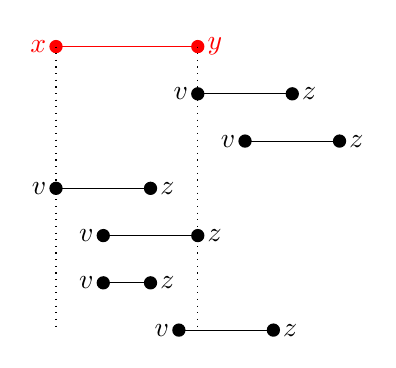
\begin{tikzpicture}[scale=1.2]
\draw[draw=none,use as bounding box](-0.3,0.2) rectangle (3.3,-3.1);
\coordinate [label=left:\textcolor{red}{$x$}] (A0) at (0,0);
\coordinate [label=right:\textcolor{red}{$y$}] (B0) at (1.5,0);
\draw[red] (A0) -- (B0);
\fill [red] (A0) circle (2pt);
\fill [red] (B0) circle (2pt);

\coordinate [label=left:$v$] (A) at (1.5,-0.5);
\coordinate [label=right:$z$] (B) at (2.5,-0.5);
\draw[black] (A) -- (B);
\fill [black] (A) circle (2pt);
\fill [black] (B) circle (2pt);

\coordinate [label=left:$v$] (A) at (2,-1);
\coordinate [label=right:$z$] (B) at (3,-1);
\draw[black] (A) -- (B);
\fill [black] (A) circle (2pt);
\fill [black] (B) circle (2pt);

\coordinate [label=left:$v$] (A) at (0,-1.5);
\coordinate [label=right:$z$] (B) at (1,-1.5);
\draw[black] (A) -- (B);
\fill [black] (A) circle (2pt);
\fill [black] (B) circle (2pt);

\coordinate [label=left:$v$] (A) at (0.5,-2);
\coordinate [label=right:$z$] (B) at (1.5,-2);
\draw[black] (A) -- (B);
\fill [black] (A) circle (2pt);
\fill [black] (B) circle (2pt);

\coordinate [label=left:$v$] (A) at (0.5,-2.5);
\coordinate [label=right:$z$] (B) at (1,-2.5);
\draw[black] (A) -- (B);
\fill [black] (A) circle (2pt);
\fill [black] (B) circle (2pt);

\coordinate [label=left:$v$] (A) at (1.3,-3);
\coordinate [label=right:$z$] (B) at (2.3,-3);
\draw[black] (A) -- (B);
\fill [black] (A) circle (2pt);
\fill [black] (B) circle (2pt);

\coordinate (A1) at (0,-3);
\coordinate (B1) at (1.5,-3);
\draw[dotted] (A0) -- (A1);
\draw[dotted] (B0) -- (B1);
\end{tikzpicture}}\\

\textsc{meets} & $\hsA$ (after) & $[x,y]\mathpzc{R}_A[v,z]\iff y=v$ &\\

\textsc{before} & $\hsL$ (later) & $[x,y]\mathpzc{R}_L[v,z]\iff y<v$ &\\

\textsc{started-by} & $\hsB$ (begins) & $[x,y]\mathpzc{R}_B[v,z]\iff x=v\wedge z<y$ &\\

\textsc{finished-by} & $\hsE$ (ends) & $[x,y]\mathpzc{R}_E[v,z]\iff y=z\wedge x<v$ &\\

\textsc{contains} & $\hsD$ (during) & $[x,y]\mathpzc{R}_D[v,z]\iff x<v\wedge z<y$ &\\

\textsc{overlaps} & $\hsO$ (overlaps) & $[x,y]\mathpzc{R}_O[v,z]\iff x<v<y<z$ &\\

\hline
\end{tabular}
%}
\end{sidewaystable}
Table~\ref{allen} depicts 6 of the 13 Allen's relations
together with the corresponding $\HS$ (existential) modalities. 
The other 7 are equality and the 6 inverse (symmetrical) relations 
(given a binary relation $\mathpzc{R}$, its inverse $\overline{\mathpzc{R}}$ is such that $b \overline{\mathpzc{R}} a$ iff $a \mathpzc{R} b$). 

The language of $\HS$ features a set of proposition letters $\Prop$, the Boolean connectives $\neg$ and $\vee$, and a temporal modality for each of the (non trivial) Allen's relations, namely, $\hsA$, $\hsL$, $\hsB$, $\hsE$, $\hsD$, $\hsO$, $\hsAt$, $\hsLt$, $\hsBt$, $\hsEt$, $\hsDt$ and $\hsOt$.
$\HS$ formulas are defined by the following grammar:
\begin{equation*}
    \psi ::= p \;\vert\; \neg\psi \;\vert\; \psi \vee \psi \;\vert\; \hsX\psi \;\vert\; \hsXt\psi, \ \ \mbox{ with } p\in\mathpzc{AP},\; X\in\{A,L,B,E,D,O\}.
\end{equation*}
%
Throughout the thesis, we will make use of the standard abbreviations of propositional logic, e.g., we write $\psi \wedge \phi$ for $\neg(\neg\psi \vee \neg\phi)$, $\psi \rightarrow \phi$ for $\neg \psi \vee \phi$, $\psi \leftrightarrow \phi$ for $\left(\psi \rightarrow \phi\right)\wedge\left(\phi \rightarrow \psi\right)$, $\true$ (true) for $p\vee\neg p$, and $\false$ (false) for $\neg\true$.

For all $X\in\{A,L,B,E,D,O\}$, the (dual) universal modalities $\hsXu\psi$ and $\hsXtu\psi$ are defined as $\neg\hsX\neg\psi$ and $\neg\hsXt\neg\psi$, respectively. 
We denote by $\mathsf{X_1\cdots X_n}$ the fragment of $\HS$, closed under Boolean connectives, that features (existential and universal) modalities for $\langle X_1\rangle,\ldots, \langle X_n\rangle $ only.

W.l.o.g., we assume the \emph{non-strict semantics} of $\HS$, which admits intervals consisting of a single point.\footnote{All the results we prove in this thesis hold for the strict semantics as well, which disallows point-intervals.} Under such an assumption, all $\HS$ modalities can be expressed in terms of
%$\hsA$, $\hsB, \hsE$, 
%%and the transposed modalities 
%$\hsAt, \hsBt$, and $\hsEt$ 
$\hsB, \hsE, \hsBt$ and $\hsEt$~\cite{HS91}.
As an example, $\hsA$ (resp., $\hsAt$) can be expressed by $\hsE$ and $\hsBt$ (resp., $\hsB$ and $\hsEt$) as 
\[\hsA \varphi= (\hsEu\bot \wedge (\varphi \vee \hsBt \varphi)) \vee \hsE (\hsEu\bot \wedge (\varphi \vee \hsBt \varphi))\] 
\[(\text{resp., } \hsAt \varphi= (\hsBu\bot \wedge (\varphi \vee \hsEt \varphi)) \vee \hsB (\hsBu\bot \wedge (\varphi \vee \hsEt \varphi))).\]
%
As for all other modalities, the next equivalences hold:
\begin{equation*}
\begin{array}{cc}
\hsL\psi=\hsA\hsA\psi & \qquad \hsLt\psi=\hsAt\hsAt\psi \\ 
\hsD\psi=\hsB\hsE\psi= \hsE\hsB\psi & \qquad \hsDt\psi=\hsBt\hsEt\psi =\hsEt\hsBt\psi \\ 
\hsO\psi=\hsE\hsBt\psi & \qquad \hsOt\psi=\hsB\hsEt\psi .
\end{array}
\end{equation*}
We also use the auxiliary operator $\hsG$ of $\HS$ (and its dual $\hsGu$), which allows one to select  arbitrary subintervals of a given interval, and is defined as: $\hsG\psi= \psi \vee \hsB\psi \vee \hsE\psi \vee \hsB\hsE\psi$.

$\HS$ can thus be seen as a multi-modal logic with   
four primitive modalities
and its semantics can be defined over a multi-modal structure, called \emph{abstract interval model}, where intervals are treated as atomic objects and Allen's relations as 
%simple 
binary relations between pairs of intervals.
Since later we will focus on some $\HS$ fragments not including some of the primitive modalities, we consider explicitly both $\hsA$ and $\hsAt$ in addition to $\hsB, \hsE, \hsBt$ and $\hsEt$.

\begin{definition}[Abstract interval model]\label{def:AIM}
An \emph{abstract interval model} is a tuple \[\mathpzc{A}=(\mathpzc{AP},\mathbb{I},A_\mathbb{I},B_\mathbb{I},E_\mathbb{I},\sigma),\] where:
\begin{itemize}
    \item $\mathpzc{AP}$ is a finite set of proposition letters;
    \item $\mathbb{I}$ is a possibly infinite set of atomic objects (worlds);
    \item $A_\mathbb{I}$, $B_\mathbb{I}$, $E_\mathbb{I}$ are three binary relations over $\mathbb{I}$;
    \item $\sigma:\mathbb{I}\mapsto 2^{\mathpzc{AP}}$ is a (total) labeling function, which assigns a set of proposition letters to each world.
\end{itemize}
\end{definition}
Intuitively, in the interval setting, $\mathbb{I}$ is a set of intervals, $A_\mathbb{I}$, $B_\mathbb{I}$, and $E_\mathbb{I}$ are interpreted as Allen's interval relations $A$ (\emph{meets}), $B$
(\emph{started-by}), and $E$ (\emph{finished-by}), respectively, and $\sigma$ assigns to each interval the set of proposition letters that hold over it.

\begin{definition}[$\HS$ semantics]\label{def:satisfaction}
Given an abstract interval model $\mathpzc{A}=(\mathpzc{AP},\mathbb{I},A_\mathbb{I},B_\mathbb{I},E_\mathbb{I}, \sigma)$
and a world $I\in\mathbb{I}$, the truth of an $\HS$ formula over $I$ is defined by induction on the structural complexity of the formula as:
\begin{itemize}
    \item $\mathpzc{A},I\models p$ iff $p\in \sigma(I)$, for any proposition letter $p\in\mathpzc{AP}$;
%    \item $\mathpzc{A},I\models \top$ and $\mathpzc{A},I\not\models \bot$
    \item $\mathpzc{A},I\models \neg\psi$ iff it is not true that $\mathpzc{A},I\models \psi$ (also denoted as $\mathpzc{A},I\not\models \psi$);
%    \item $\mathpzc{A},I\models \psi \wedge \varphi$ iff $\mathpzc{A},I\models \psi$ and %$\mathpzc{A},I\models \varphi$;
        \item $\mathpzc{A},I\models \psi \vee \varphi$ iff $\mathpzc{A},I\models \psi$ or $\mathpzc{A},I\models \varphi$;
    \item $\mathpzc{A},I\models \hsX\psi$, for $X \in\{A,B,E\}$, iff there exists $J\in\mathbb{I}$ such that $I\, X_\mathbb{I}\, J$ and $\mathpzc{A},J\models \psi$;
    \item $\mathpzc{A},I\models \hsXt\psi$, for $\overline{X} \in\{\overline{A},\overline{B},\overline{E}\}$, iff there exists $J\in\mathbb{I}$ such that $J\, X_\mathbb{I}\, I$ and $\mathpzc{A},J\models \psi$.
\end{itemize}
\end{definition}

\emph{Satisfiability} (SAT) and \emph{validity} are defined in the usual way: an $\HS$ formula $\psi$ is satisfiable if there exists an interval model $\mathpzc{A}$ and a world (interval) $I$ such that $\mathpzc{A},I\models \psi$. Moreover, $\psi$ is valid if $\mathpzc{A},I\models \psi$ for all worlds (intervals) $I$ of every interval model $\mathpzc{A}$. 


%%%%%%%%%%%%%%%%%%%%%%%%%%%%%%%%%%

In~\cite{HS91}  
it was shown that the \emph{validity problem} for $\HS$ interpreted
over any class of linear orders that contains at least one linear order with an
infinite ascending or descending sequence of points,
 is \emph{undecidable} (more precisely, r.e.\ hard).
For example, it is undecidable over $\mathbb{N}$ (the natural numbers), $\mathbb{Z}$ (the integers), $\mathbb{Q}$ (the rationals) and $\mathbb{R}$ (the reals), 
as well as over the classes of all linear orders, all dense linear orders, and all discrete linear orders.
%
Moreover, over any class of \emph{Dedekind complete} ordered structures containing at least an order with an infinite ascending sequence,
it is $\Pi_1^1$-hard (i.e., not recursively axiomatizable). This is true, e.g., over $\mathbb{N}$, $\mathbb{Z}$,  and $\mathbb{R}$, being Dedekind complete. 

The authors of~\cite{DBLP:journals/eatcs/MonicaGMS11} state that:
\begin{quote}
[\dots] so general undecidability results about $\HS$ are given in~\cite{HS91}
that for a long time it was considered unsuitable for practical applications and
attracted little interest among computer scientists.  
\end{quote}

Since then, a lot of work has been done on the SAT
problem for \emph{fragments} of $\HS$, which showed that undecidability rules also over
them~\cite{Bresolin2008,DBLP:conf/time/BresolinMGMS09,DBLP:journals/amai/BresolinMGMS14,DBLP:conf/asian/Lodaya00,DBLP:journals/fuin/MarcinkowskiM14}. As an example, the fragment $\BE$ (i.e., formulas of $\HS$ with $\hsB$ and $\hsE$ modalities only) is undecidable, again, over the class of all linear orders, over all dense linear orders, discrete linear orders and finite linear orders~\cite{DBLP:conf/asian/Lodaya00}.

The reason for these undecidability results must be ascribed to the very nature of purely interval-based temporal reasoning, where 
proposition letters are interpreted on 
intervals (and not on points): 
the set-theoretic interpretation of an
$\HS$ formula in a model is a set of abstract intervals, that is, a set of pairs of points (a binary relation over the underlying linear order).
%
Automata-based methods, founded for instance on Büchi and Rabin theorems (implying decidability of MSO theories of various linear orders and trees), do not apply here, as SAT and validity for ITLs are
dyadic, and not monadic. New approaches for proving decidability of $\HS$ fragments with genuinely interval-based semantics were needed.

Meanwhile, several modifications or restrictions, essentially reducing the interval-based semantics to
a point-based one,  were proposed to remedy the problem and obtain decidable systems. As an example, already in~\cite{digital_circuits_thesis} Moszkowski showed that the decidability of the (otherwise undecidable) logic $\PITL$ can be recovered by constraining  proposition letters to be
point-wise and defining truth of an interval as truth on its initial point (\emph{locality principle}). 

The bleak picture started lightening up later, with the discovery of several non-trivial cases of decidable fragments of $\HS$~\cite{DBLP:journals/logcom/BresolinGMS10, DBLP:journals/apal/BresolinGMS09, BMSS11, MPS10,MPSS10,DBLP:conf/time/MontanariS12INS, DBLP:conf/tableaux/BresolinMSS11INS}, including the \emph{interval logic of temporal
neighbourhood} $\AAbar$ and the \emph{temporal logic of sub-intervals} $\D$. %
In particular, the former was shown to be decidable over the class of 
all linear orders, of all dense, of all discrete, and of all finite linear orders;%
\footnote{It is also worth mentioning the decidable metric extension of the fragment $\AAbar$ called MPNL, studied in~\cite{DBLP:journals/sosym/BresolinMGMS13,DBLP:conf/ecai/BresolinMGMS10,DBLP:journals/corr/abs-1106-1241}, that features 
special atomic propositions representing integer constraints (equalities  and  inequalities) on the length of the intervals over which they are predicated.}
as for the latter, the situation is more involved:
$\D$ is \emph{decidable} over all dense linear orders, \emph{undecidable} over discrete linear orders and finite linear orders~\cite{DBLP:journals/fuin/MarcinkowskiM14}, 
and it is not known whether it is decidable or not in the case of all linear orders.
%
Some other fragments, such as $\B\Bbar$ and $\E\Ebar$, have actually a \emph{point-based} semantics: one of the endpoints of every interval related to the current one can ``move'', but the other always remains fixed; as a consequence they can be polynomially translated into a basic point-based temporal logic (namely, the fragment of $\LTL$ with only the future $\Eventually$ and past $\mathsf{P}$ operators): any interval is mimicked by its only moving endpoint; it follows that $\B\Bbar$ and $\E\Ebar$ are decidable over the class of all linear orders and, in particular, $\NP$-complete~\cite{roadmap_intervals}.
%
On the other hand, another fragment, $\AAbarBBbar$, is decidable over finite linear orders, $\mathbb{Q}$, as well as over the class of
all linear orders, but undecidable over Dedekind-complete linear orders (in particular, $\mathbb{N}$ and $\mathbb{R}$)~\cite{DBLP:conf/mfcs/MontanariPS14Ratio}.
%
These snapshots on $\HS$ SAT make us conclude, with the authors of~\cite{DBLP:journals/eatcs/MonicaGMS11}, that
\begin{quote}
[\dots] the trade-off
between expressiveness and computational affordability in the family of $\HS$ fragments
is rather subtle and sometimes unpredictable, with the border between decidability and undecidability cutting right
across the core of that family.
\end{quote}

\section{The problem of MC for \HS}

Whereas, as we have seen, darkness reigns in the realm of SAT with few exceptions,
fortunately a dim light brightens the whole land of MC for $\HS$:
in this thesis, we will consider this \emph{decidable} problem,
for which a little work has been done, if compared to SAT of $\HS$ and especially to MC of point-based temporal logics.

For quite a long time, no studies on MC for $\HS$ were undertaken: the problem was finding 
suitable system models over which to interpret such an interval-based property specification language 
(clearly, this was a novel issue to face, as the SAT problem is defined more simply on linear orders).
In 2011, Dario Della Monica concluded his PhD thesis about decidability and undecidability results on SAT for $\HS$ and its fragments in this way~\cite{DarioDM:phd_thesis}:
\begin{quote}
Even if this topic [MC] has been extensively studied and successfully applied to real-world domains in the context of point-based logics, it is still quite
unexplored in the interval setting. The major difficulty concerns the problem of finding a convenient way to (finitely) represent the models to be checked.
\end{quote}

The first idea we explore in this thesis is evaluating $\HS$ formulas on (very standard) system models, consisting essentially in \emph{labeled graphs}, called finite \emph{Kripke structures} (which will be formally defined later), making it
possible to check the correctness of the behavior of systems with respect to 
meaningful interval properties. 
In order to verify interval properties of computations, one needs to collect 
information about the states of a system into computation stretches.
To this end, each finite path (i.e., a \emph{trace}) in a Kripke structure is interpreted as an interval, 
and its labeling is defined on the basis of the labeling of the states composing it, initially
according to the \emph{homogeneity assumption}~\cite{Roe80}, which enforces a proposition letter $p$ to hold on an interval $I$ if and only if $p$ holds on all the subintervals of $I$.
Such an assumption is fairly natural for many applications; moreover, it easily enables us to 
interpret an \emph{interval-based} property specification language on a model which is \emph{point-based} (as a matter of fact, Kripke structures make explicit how a system evolves \emph{state-by-state}, and describe which are the atomic properties that hold true at every single state).

Then we devote our efforts to 
relaxing homogeneity.
For the purpose, we investigate the possibility of using regular expressions to define the labeling of proposition letters over intervals in terms of the component states (as we will see, homogeneity can be trivially encoded by regular expressions, as a particular case). This impacts on the complexity of MC for \HS\ and its fragments, and on the expressiveness of the logic as well. 
Another possibility is completely abandoning Kripke structures in favour of different, \emph{inherently interval-based} system models: \emph{timelines}, structures that have been fruitfully exploited in temporal planning for quite a long time, are employed in this thesis in a different way: more expressive than Kripke structures, they 
allow us to directly describe systems in terms of their \emph{interval-based behaviour and properties},
paving the way for a more general interval-based MC.

\section{Organization of the thesis}
Let us now take a deeper look at the contents of the thesis, while presenting its organization.
\begin{enumerate}
    \item In the next chapter---which starts Part~\ref{part:HShomo}---we show that finite Kripke structures can be suitably mapped into
abstract interval models, 
whose worlds are all the possible traces of the former.
However, since Kripke structures may have loops and thus infinitely many traces, abstract interval models feature, in 
general, an infinite domain. 
In order to devise a MC procedure for $\HS$ over finite Kripke
structures---hence showing the decidability of MC for $\HS$---we prove a small model theorem stating that, given an $\HS$ 
formula $\psi$ and a finite Kripke structure $\Ku$, there exists a \emph{finite}
interval model which is equivalent to the one induced by $\Ku$ with respect 
to the satisfiability of $\psi$.
The main technical ingredients are $(i)$~the definition of a suitable equivalence relation 
over traces of $\Ku$, which is parametric in the nesting 
depth of modalities $\hsB$ and $\hsE$ in $\psi$, and $(ii)$~the proof that 
the resulting quotient structure is finite and equivalent to the one induced by 
$\Ku$ with respect to the satisfiability of $\psi$.

The chapter is concluded showing that the problem does not provably admit any polynomial-time decision procedure (as it is \EXPSPACE-hard). For this reason, 
\item
in the subsequent chapters of Part~\ref{part:HShomo} we focus on fragments of \HS , which 
feature considerably better complexities---from \EXPSPACE, down to \Psp\ and to low levels of the polynomial hierarchy. Nevertheless, they have the ability to capture meaningful interval properties of state transition systems.
We describe several MC algorithms, tailored to the specific fragments being considered, which feature as building blocks concepts and techniques different from one another (e.g., small model properties, trace contractions, Boolean circuits with oracles, finite state automata,\ldots). Most of the times, we also prove lower bounds matching the complexity of MC algorithms.

Moreover, we study the expressive power of $\HS$ in MC, in comparison with that of the standard point-based logics $\LTL$, $\CTL$ and $\CTLStar$, still under homogeneity.
Additionally, we introduce some \emph{semantic variants} of \HS\  and evaluate their expressiveness and succinctness with respect to the aforementioned point-based logics.

\item
The homogeneity assumption is relaxed in Part~\ref{part:HSrelaxhomo}: as we have anticipated, at first we still consider Kripke structures as system models, but we 
use regular expressions to define the labeling of proposition letters over intervals in terms of the component states.
In particular, MC for \HS\ extended with regular expressions remains still decidable: this result is proved via a (non completely standard) automata-theoretic approach.

As for the fragments of \HS, the MC problem for \lq\lq small\rq\rq\ ones features an increased (\Psp) complexity, whereas formulas of other, more expressive fragments, can be checked at no extra computational cost (w.r.t.\ the homogeneous case).
Such complexity results are achieved by heavily exploiting \emph{non-deterministic} and \emph{alternating} algorithms.

\item
Finally, in Part~\ref{part:timelines} we
consider the \emph{timeline-based MC problem},
where system models are given by the aforementioned \emph{timelines},
and the property specification language is the logic $\mathsf{MITL}$: the choice of replacing $\HS$ with the latter is justified by the need for a \emph{timed} logic, appropriate to be interpreted over timelines, where the dimension of time is essential. 

Most of Part~\ref{part:timelines} will be actually devoted to the study of the so-called \emph{timeline-based planning problem} over \emph{dense temporal domains}:
first, such problem can be considered as a necessary condition for MC, the former playing the role of a \lq\lq feasibility check\rq\rq\ of the system description (as a matter of fact, whereas Kripke structures are \lq\lq extensive\rq\rq\ system descriptions, timelines are not, given the presence of constraint rules which must be checked for satisfiability). 
Moreover, dense time domains (as opposed to discrete ones, which are standard in planning) are necessary to avoid discreteness in system descriptions, that can be abstracted at a higher level, enabling us to express really interval-based properties of systems.
Since, in its full generality, timeline-based planning over dense domains is, unfortunately, undecidable, suitable restrictions on timelines are identified at the beginning of Part~\ref{part:timelines} in order to recover its decidability, and finally deal with timeline-based MC.

\end{enumerate}
